\documentclass{amsart}[12pt]
\usepackage{amsmath, amsfonts, tikz, natbib, array}
\usetikzlibrary{patterns}
\oddsidemargin=0in \evensidemargin=0in
\textwidth=6.6in \textheight=8.7in

\title{Triangular map projections}
\author{B R S Recht}
\date{April 202X}

\begin{document}
\maketitle
\tableofcontents

\section{Introduction}
A small but persistent trend in creating world maps has been to map onto a polyhedron, and then unfold the polyhedron into a flat polyhedral net. An example is Buckminster Fuller's (second) Dymaxion map, based on an icosahedron.\cite{gray94} Snyder's equal-area map projection enabled equal-area polyhedral maps.\cite{snyder92} Conformal map projections exist for all polyhedra, although their calculation may be involved.\cite{lee1976conformal} The inverse of each map projection can be used to inscribe a regular grid on a sphere, termed a geodesic grid (after Fuller's geodesic domes) or discrete global grid.\cite{williamson}\cite{sahr98}.

Projections for the cube, the dodecahedron, and other polyhedra with non-triangular faces almost all divide the faces into triangles. The exception are those that use the gnomonic projection directly (which transforms all spherical polygons within a hemisphere into planar polygons), the conformal projections (which are specific to each polyhedron) and the quadrilateral projection similar to Fuller's presented in \cite{crider09}. Therefore, this paper limits itself to triangular map projections. 

There are several qualities that can be considered for a polyhedral map.
* Discontinuities, which mostly depend on the polyhedron and how it is unfolded.
* Flation; distortion of area. 
* Angle distortion.
* Cusps; lines or curves where the projection introduces a sharp bend in intersecting lines, and the map projection fails to be differentiable. We make a distinction between interior cusps, which lie within the interior of a polyhedral face, and edge cusps, which lie on the edges between faces.
* Symmetry, in a sense that will be defined more clearly later.

For example, conformal polyhedral map projections have no angle distortion but heavy flation, with areas shrinking to zero near the vertexes. Being conformal, they do not have cusps, either interior or edge. The Dymaxion map uses a compromise projection, either the gnomonic or another developed by Fuller, that balances flation with angle distortion without eliminating either. It has edge cusps but not interior. Snyder's equal-area projection has high angle distortion, and also introduces interior cusps lying on the lines between a face's center and its vertices. Snyder divides a polyhedral face into triangles, and those interior cusps are the edge cusps of the 

We will focus on the faces of regular polyhedra, specifically the icosahedron, but not to exclusion. We do exclude hemispherical triangles from consideration, in part because many map projections fail 


In this text, map projections between spherical and Euclidean
triangles will be discussed. Some of these are existing map projections, or
extensions of those, while some are new compromise map projections. Some
projections where only the forward or inverse transformation is known in close-
form are included. An attempt is made to generalize projections to irregular
triangles and to be able to project a portion of the exterior of the triangle
as well.

\begin{table}
\begin{tabular}[]{l l}
  Name & Reference / Equation \\
  Gnomonic & \cite{snyder87}  \\
  Conformal & \cite{lee1976conformal} \\
  Snyder equal-area & \cite{snyder92} \\
  Small circle equal-area & \cite{leeuwen2006} \\
  Fuller & \cite{crider08} \\
  Areal & Eqs. \ref{eq:sphericalarealfwd}, \ref{eq:sphericalarealinv} \\
  Bisect Area & Eq. ? \\
  Bisect Distance & Eq. ? \\  
  Linear Combination & Eq. ?\\  
  Symmetrized Snyder & Eq. ? \\
  Symmetrized small circle & Eq. ? \\
  Single-variable optimizations & Table x \\
  Multi-variable optimizations & Table y  
\end{tabular}
\caption{Map projections used or introduced in this text.}
\label{fig:projs}
\end{table}

\section{Preliminaries}
Let $(u,v)$ be a vector in $\mathbb R^2$, and $\zeta = u + i v$ be the
corresponding complex number in $\mathbb C$ or the Riemann sphere $\mathbb C
\cup \{\infty\}$. Which notation is used will depend on the mapping:
conformal maps are best expressed in terms of complex variables.

\subsection{Vectors on the sphere}
Some of the map projections to be discussed are better expressed
in terms of a vector rather than latitude and longitude. This text will only
cover pertinent details: a fuller description can be found in e.g. \cite{strang80}.

Let $\phi \in [-\frac{\pi}{2}, \frac{\pi}{2}]$ be latitude, and
$\lambda \in (-\pi, \pi]$ be longitude. Let $\mathbf v = (x, y, z)$ be a vector
in $\mathbb R^3$ and $\mathbf{\hat{v}} = (x, y, z)$ be a unit vector on the
sphere $S^2$ such that $\| \mathbf{\hat{v}} \| = \sqrt{x^2 + y^2 +z^2} = 1$.
To convert from latitude and longitude to a unit vector:
\begin{equation}
  \mathbf{\hat{v}} = \left(\sin (\phi), \sin (\lambda) \cos (\phi),
  -\cos (\lambda) \cos (\phi) \right)
\end{equation}
To convert from the unit vector $\mathbf{\hat{v}}$ to latitude and longitude:
\begin{equation}\begin{split}
  \phi &= \arcsin (x) = \arctan (x, \sqrt{y^2 + z^2}) \\
  \lambda &= \arctan (y, -z)
\end{split}\end{equation}

\subsection{Barycentric coordinates and affine transformations}

Barycentric coordinates are real numbers $\beta_1, \beta_2, \beta_3$ such that $\sum^3_{i=1} \beta_i = 1$. Given a triangle in Euclidean space with vertices $\mathbf v_1, \mathbf v_2, \mathbf v_3$, the corresponding vertex is given by $\mathbf v = \sum^3_{i=1} \beta_i \mathbf v_i$. Given $\mathbf v$ and $\mathbf v_i$, $\beta_i$ can be found by e.g. solving the linear system of $\beta_1 + \beta_2 + \beta_3 = 1$ and $\mathbf v = \sum^3_{i=1} \beta_i \mathbf v_i$. $\beta_i$ are all positive on the interior of the triangle. If a point lies on an edge opposite vertex $i$, then $\beta_i$ is zero. (If it lies beyond the edge, then $\beta_i < 0$.)

Barycentric coordinates can be thought of as a special form of affine transformation. Affine transformations are combinations of reflection, scaling, rotation, shearing, and translation. This can be expressed as $\mathbf v = \mathbf A [u, v]^T + v_0$, where $\mathbf A$ is a matrix. It is generally desirable to avoid the degenerate case $|\mathbf A| = 0$, which maps the plane to a line. An affine transformation which consists only of scaling, rotation, and translation, so that it preserves angles, is called a conformal affine transformation.

\section{Map projections}

Let us begin by mentioning some preexisting triangular projections. As these are already well-documented in the literature, we will not repeat their formulas here.

The gnomonic projection was known to the ancient Greeks, and appears in most books on map projections, including \cite{snyder87}. It has the property that arcs of great circles are transformed into lines on the plane, so it in fact transforms every triangle contained within a hemisphere to some triangle in the plane.

Lee's 1976 monograph on conformal map projection \cite{lee1976conformal} remains the best available description of conformal triangular map projections.

\cite{crider08} gives the most complete description of a map projection used by Fuller for his Dymaxion map, here referred to as Fuller's projection.

\subsection{Snyder equal-area}
\cite{snyder92}\cite{leeuwen2006}

\cite{lambers}\cite{patt}

\subsection{Small circle equal-area}
\cite{leeuwen2006} introduces a map projection we'll refer to as the Small circle equal-area projection. It is similar to the Snyder equal-area projection.

\subsection{Spherical areal}
\begin{figure}%[!htbp]
	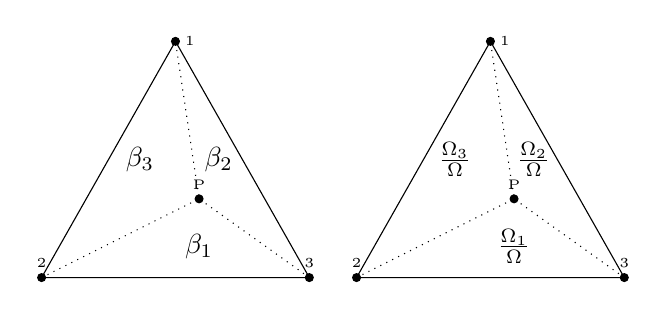
\begin{tikzpicture}
		\draw (0, 0) -- (1.7,3) -- (3.4, 0) -- (0, 0) ;
		\draw[fill] (1.7, 3) circle [radius=0.05] node[anchor=west] {\tiny 1};
		\draw[fill] (0, 0) circle [radius=0.05] node[anchor=south] {\tiny 2};
		\draw[fill] (3.4, 0) circle [radius=0.05] node[anchor=south] {\tiny 3};
		\draw[fill] (2, 1) circle [radius=0.05]
		node[anchor=south] {\tiny P};
		\draw[dotted] (0,0) -- (2,1) -- (1.7,3);
		\draw[dotted] (3.4, 0) -- (2,1);
		\node at (2,0.4) {$\beta_1$};
		\node at (2.25,1.5) {$\beta_2$};
		\node at (1.25,1.5) {$\beta_3$};		
		
		\draw (4, 0) -- (5.7,3) -- (7.4, 0) -- (4, 0) ;
		\draw[fill] (5.7, 3) circle [radius=0.05] node[anchor=west] {\tiny 1};
		\draw[fill] (4, 0) circle [radius=0.05] node[anchor=south] {\tiny 2};
		\draw[fill] (7.4, 0) circle [radius=0.05] node[anchor=south] {\tiny 3};
		\draw[fill] (6, 1) circle [radius=0.05]		node[anchor=south] {\tiny P};
		\draw[dotted] (4,0) -- (6,1) -- (5.7,3);
		\draw[dotted] (7.4, 0) -- (6,1);
		\node at (6,0.4) {$\frac{\Omega_1}{\Omega}$};
		\node at (6.25,1.5) {$\frac{\Omega_2}{\Omega}$};
		\node at (5.25,1.5) {$\frac{\Omega_3}{\Omega}$};		
	\end{tikzpicture}
	\caption{Spherical areal projection. Left: Barycentric coordinates in the plane. Right: Areas  inside the spherical triangle.}
	\label{fig:sphericalareal}
\end{figure}
The spherical areal projection makes use of the relationship between barycentric coordinates and area. Refer to Figure \ref{fig:sphericalareal}, first the Euclidean triangle on the left. Let $\hat{\mathbf v}_i$ be the vertices of the triangle and $\hat{\mathbf v}_P$ be the projected point. A property of barycentric coordinates is that $\beta_i$ equals the ratio of the area of the small triangle opposite vertex $i$ and the area of the large triangle. This remains true for points outside the triangle if signed areas are used.

Draw an analogous spherical triangle as on the right of Figure \ref{fig:sphericalareal}. Let $\Omega_i$ designate the geodesic area of the small triangle opposite of vertex $i$, and $\Omega$ designate the area of the large triangle. A forward map projection can be defined by setting the two ratios of areas to be equal:

\begin{equation}\label{eq:sphericalarealfwd}
	\beta_i = \frac{\Omega_i}{\Omega}
\end{equation}

This can easily be shown to map the vertices of the large spherical triangle to the vertices of the large Euclidean triangle, and points on the edge of the spherical triangle to the corresponding edge of the Euclidean triangle. It is also invariant under cyclic permutation. This projection can be applied to ellipsoids, although given that the projection is neither conformal nor equal-area, there is little reason in practical cartography not to use the spherical approximation. More generally it can be applied to any surface where area is well-defined, and therefore can be compared to the azimuthal equidistant projection, which is a special case of the exponential map in Riemannian geometry.

In the spherical approximation, this projection has an inverse. First note that the area $\Omega$ of a spherical triangle can be given in terms of unit vectors of its vertices as so:\cite{oosterom}\cite{eriksson}
\begin{equation}
\tan(\Omega/2) = \frac{|\mathbf{\hat{v}_1} \cdot
       \mathbf{\hat{v}}_2 \times \mathbf{\hat{v}}_3|}
       {1+\mathbf{\hat{v}}_1\cdot \mathbf{\hat{v}}_2+\mathbf{\hat{v}}_2
       \cdot \mathbf{\hat{v}}_3+\mathbf{\hat{v}}_3\cdot \mathbf{\hat{v}}_1}
\end{equation}

There are some quantities that depend only on the larger triangle, not the point to be projected:
\begin{equation}\begin{split}		
		a_i & = \mathbf v_{i-1} \cdot \mathbf v_{i+1} \\
		b_i & = \frac{a_{i-1} + a_{i+1}}{1 + a_i}\\
		\tau &= \tan\left(\frac{\Omega}{2}\right) \\
\end{split}\end{equation}
With that, start with $\beta_i$ as givens, and proceed as follows. While lengthy, this set of formulas consists only of scalar and vector arithmetical operations and the $\tan$ function.
%https://math.stackexchange.com/questions/1151428/point-within-a-spherical-triangle-given-areas/3189416#3189416

\begin{equation}\label{eq:sphericalarealinv}\begin{split}		
\Omega_i & = \beta_i \Omega \\	
\tau_i &= \tan\left(\frac{\Omega_i}{2}\right) \\
t_i &= \frac{\tau_i}{\tau} \\
c_i &= \frac{t_i}{(1+b_i) + (1-b_i) t_i} \\
f_i &= \frac{c_i}{1 - c_1 - c_2 - c_3} \\
\mathbf v_P &= \sum^3_{i=1} f_i \mathbf v_i = \frac{\sum^3_{i=1} c_i \mathbf v_i }{ 1 - \sum^3_{i=1} c_i }
\end{split}\end{equation}

\subsection{Bisect Area}
This projection also makes use of area.
\begin{figure}%[!htbp]
	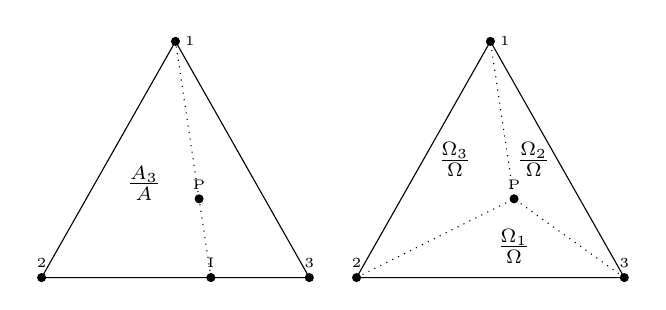
\begin{tikzpicture}
		\draw (0, 0) -- (1.7,3) -- (3.4, 0) -- (0, 0) ;
		\draw[fill] (1.7, 3) circle [radius=0.05] node[anchor=west] {\tiny 1};
		\draw[fill] (0, 0) circle [radius=0.05] node[anchor=south] {\tiny 2};
		\draw[fill] (3.4, 0) circle [radius=0.05] node[anchor=south] {\tiny 3};
		\draw[fill] (2, 1) circle [radius=0.05]
		node[anchor=south] {\tiny P};
		\draw[dotted] (2.15,0) -- (1.7,3);
		\draw[fill] (2.15, 0) circle [radius=0.05] node[anchor=south] {\tiny I};
		\node at (1.3,1.2) {$\frac{A_3}{A}$};		
		
		\draw (4, 0) -- (5.7,3) -- (7.4, 0) -- (4, 0) ;
		\draw[fill] (5.7, 3) circle [radius=0.05] node[anchor=west] {\tiny 1};
		\draw[fill] (4, 0) circle [radius=0.05] node[anchor=south] {\tiny 2};
		\draw[fill] (7.4, 0) circle [radius=0.05] node[anchor=south] {\tiny 3};
		\draw[fill] (6, 1) circle [radius=0.05]		node[anchor=south] {\tiny P};
		\draw[dotted] (4,0) -- (6,1) -- (5.7,3);
		\draw[dotted] (7.4, 0) -- (6,1);
		\node at (6,0.4) {$\frac{\Omega_1}{\Omega}$};
		\node at (6.25,1.5) {$\frac{\Omega_2}{\Omega}$};
		\node at (5.25,1.5) {$\frac{\Omega_3}{\Omega}$};		
	\end{tikzpicture}
	\caption{Bisect projection. Left: Barycentric coordinates in the plane. Right: Areas  inside the spherical triangle.}
	\label{fig:bisect}
\end{figure}

\begin{equation}
	A_1 = \frac{\beta_1}{1-\beta_2}
\end{equation}

\begin{equation}
	\begin{bmatrix}
		1 & A_1 & 0 \\
		0 & 1 & A_2 \\
		A_3 & 0 & 1
	\end{bmatrix}
	\begin{bmatrix}
		\beta_1 \\ \beta_2 \\ \beta_3
	\end{bmatrix} =
	\begin{bmatrix}
		A_1 \\ A_2 \\ A_3
	\end{bmatrix}
\end{equation}

\begin{equation}
	\beta_1 = y^2  x^2 + z^2  x^2 - y^2  z^2
	- x  y^2 + z  y^2
	- 2yx^2 - xz^2 + yz^2 + x^2
	+ 3yx + zx - 2yz
	- 2x - y + z + 1
\end{equation}


\subsection{Bisect Distance}
This is essentially the previous projection with the areas replaced by distance along each edge.

\subsection{Linear combination}

Let $f_i (\mathbf v)$ be a sequence of map projections from a spherical
polygon $R_s$
to a spherical polygon $R_e$.
Let $\mathbf v_i$ be the
vertices of the spherical polygon. Furthermore, require that $f_i(\mathbf v_j)$
takes the same value for all $i$ and $j$: the projections all maintain the same
orientation of polygon. Then, let $w_i$ be a sequence of weights, possibly
negative, such that $\sum w_i = 1$. It can be easily demonstrated that
$g(\mathbf v) = \sum w_i f_i(\mathbf v)$ is also a map projection from $R_s$ to
$R_e$. (This holds whether we think of $R_e$ in terms of barycentric coordinates
or a planar Euclidean polygon.)

If any individual $f_i(\mathbf v)$ has cusps, $g(\mathbf v)$ will generally also have cusps in the same place. 

Unfortunately, $g(\mathbf v)$ generally does not have a closed-form inverse, even if all
of the contributing $f_i(\mathbf v)$ do.

\section{Analysis}

\section{Conclusion}

\section{Acknowledgments}
Thank you to Achille Hui for deriving Equation \ref{eq:sphericalarealinv} from a much more complicated form.

\bibliographystyle{plain}
\bibliography{../references}

\end{document}
